\newpage
\section{Integrator stuff}
\label{sec:app_integrator}

ToDo: Improve interface for breakpoints (redesign?)

let's check out another feature of eMolfon, the integrator visualizer! This will let us view the visualization of the created
triple model. (i.e., tracer)

\begin{itemize}

\item[$\blacktriangleright$] Right-click on \texttt{corr\_BWD.xmi} and choose ``eMoflon $\rightarrow$ Start Integrator'' which will open the window depicted in
Fig.~\ref{fig:integrator_start}.

\vspace{0.5cm}

\begin{figure}[htbp]
\begin{center}
  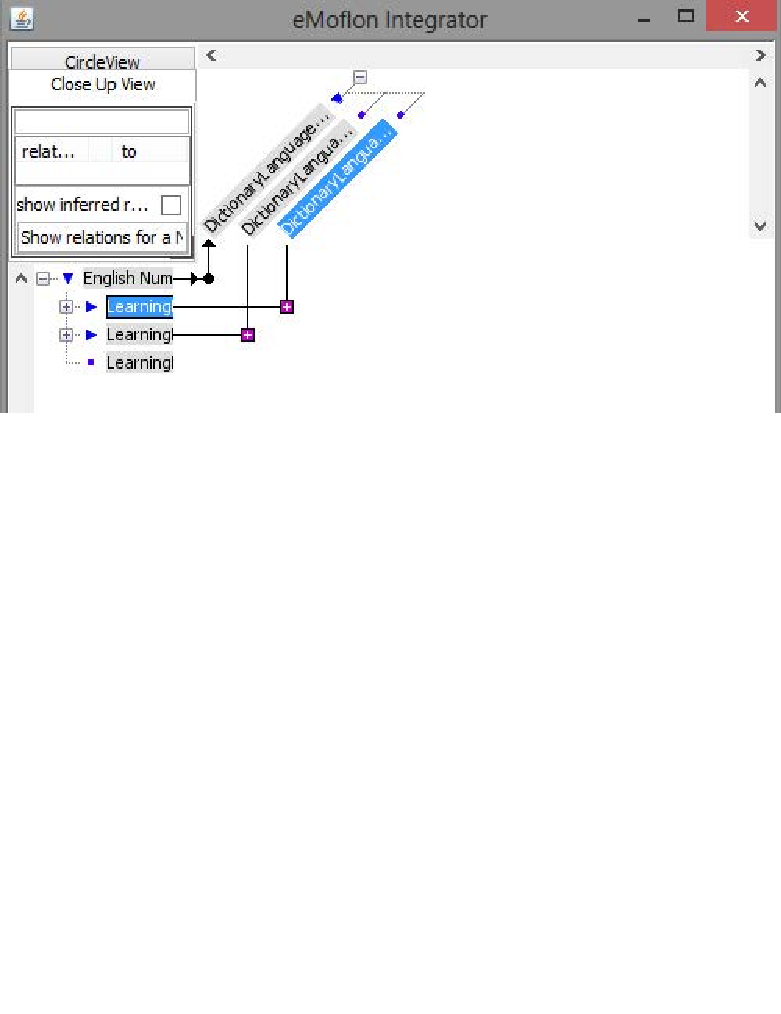
\includegraphics[width=0.7\textwidth]{integrator_start_view.pdf}
  \caption{Default view of the integrator}
  \label{fig:integrator_start}
\end{center}
\end{figure}

\item[$\blacktriangleright$] Drag and drop \texttt{protocol\_BWD.xmi} into the window. You will now see the controls explained in the lower part of the window 
(Fig.~\ref{fig:integrator_after_protocol}).

\begin{figure}[h!]
\begin{center}
  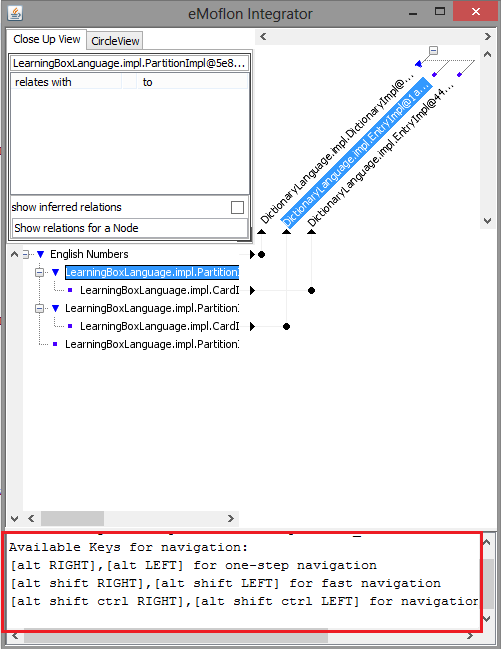
\includegraphics[width=0.6\textwidth]{integrator_after_protocol_insertion.png}
  \caption{Integrator after protocol insertion.}
  \label{fig:integrator_after_protocol}
\end{center}
\end{figure} 
\FloatBarrier

\item[$\blacktriangleright$] The integrator works as an ``offline'' debugger, working on the protocol (trace) of the transformation. You can use
\texttt{Alt+Right} to navigate forwards \emph{through} the transformation process, and \texttt{Alt+Left} to go backwards.  When you step through the
transformation, you will notice that some elements are highlighted with colours. These are the elements currently being processed. The colours have the
following definitions:
\begin{description}
  \item[Blue] The element is now about to be processed (is being ``looked at'').
	\vspace{0.25cm}
  \item[Yellow] The element cannot be transformed right now and has been queued for later transformation 
  (e.g., when transforming an Entry to a Card, the Box with partitions to put the 
  Card into must be translated first).
	\vspace{0.25cm}
  \item[Green] The object has just been created.
\end{description}

\end{itemize}

\subsection{Using breakpoints with the integrator}

((all new -- redesign interface?))
